\documentclass[tikz,border=6pt]{standalone}
\usepackage{amsmath,amssymb}
\usepackage{xcolor}
\definecolor{accent}{HTML}{A13D2C}
\definecolor{accent2}{HTML}{2B5F6B}
\definecolor{muted}{HTML}{5A564F}
\definecolor{panel}{HTML}{F8F6F0}
\definecolor{linecol}{HTML}{D8D2C4}
\definecolor{astroblue}{HTML}{1B4F72}
\definecolor{sunyellow}{HTML}{E8A33D}
\definecolor{ink}{HTML}{1E1C1A}
\definecolor{colthree}{RGB}{60,140,80}
\usetikzlibrary{calc,arrows.meta,plotmarks}
\IfFileExists{results/ch6/rv_e0.dat}{\def\datadir{results/ch6/}}{\def\datadir{../results/ch6/}}
\usepackage[T1]{fontenc}\usepackage{newpxtext,newpxmath}  % same fonts as the notes
\begin{document}
% Radial-velocity curves (v_r - gamma)/K against phase (t - t_p)/P, from code/ch6/01_rv_curves.awk.
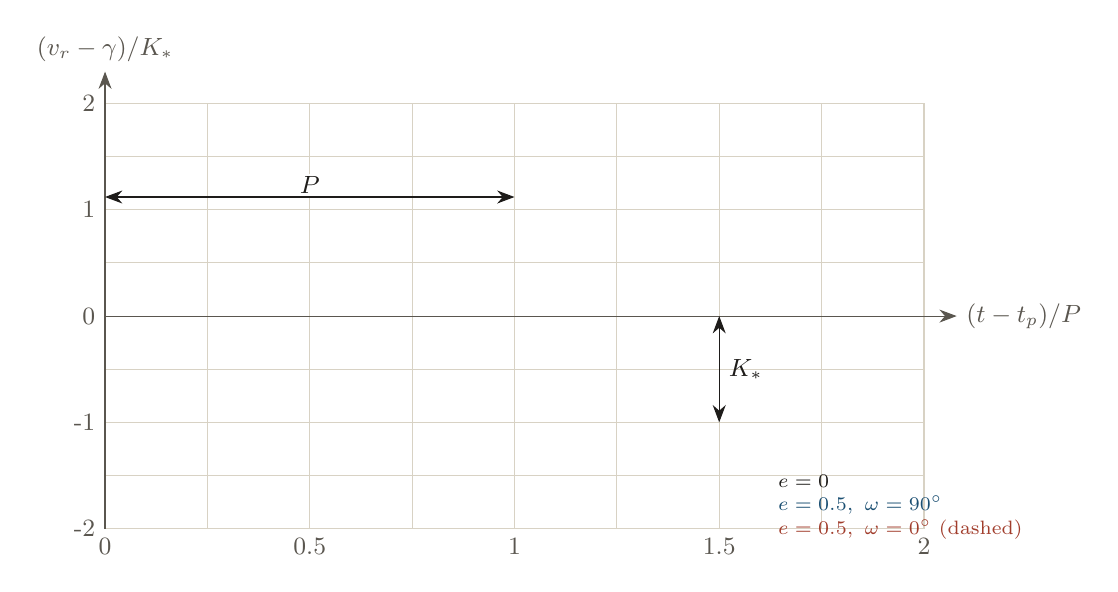
\begin{tikzpicture}[x=5.2cm,y=1.35cm, >={Stealth[length=2.2mm]}, font=\small]
  \draw[linecol] (0,-2) grid[xstep=0.25,ystep=0.5] (2,2);
  \draw[->, muted] (0,0) -- (2.08,0) node[right] {$(t-t_p)/P$};
  \draw[->, muted] (0,-2) -- (0,2.3) node[above] {$(v_r-\gamma)/K_*$};
  \foreach \x in {0,0.5,1,1.5,2} \node[below, muted] at (\x,-2) {\x};
  \foreach \y in {-2,-1,0,1,2} \node[left, muted] at (0,\y) {\y};
  \draw[ink, line width=1.0pt] plot file {\datadir rv_e0.dat};
  \draw[astroblue, line width=1.0pt] plot file {\datadir rv_e05_w90.dat};
  \draw[accent, line width=1.0pt, dashed] plot file {\datadir rv_e05_w0.dat};
  % semi-amplitude and period on the circular curve
  \draw[<->, ink] (1.5,0) -- (1.5,-1) node[midway, right] {$K_*$};
  \draw[<->, ink] (0,1.12) -- (1,1.12) node[midway, above, fill=white, inner sep=1pt] {$P$};
  \node[ink, anchor=west, font=\scriptsize] at (1.62,-1.55) {$e=0$};
  \node[astroblue, anchor=west, font=\scriptsize] at (1.62,-1.78) {$e=0.5,\ \omega=90^\circ$};
  \node[accent, anchor=west, font=\scriptsize] at (1.62,-2.01) {$e=0.5,\ \omega=0^\circ$ (dashed)};
\end{tikzpicture}
\end{document}
